\section{Data processing and basic results}
\label{section:results}

The first step in geostatistics is to build the variogram. We have used 
the omni variogram. The basic formula for the variogram:

$\gamma(h) = \frac{1}{2N(h)}\sum |z_i-z_j|^2$

Once the emprical variogram is constructed the analysis (for Simple Kriging)
proceeds as follows:

$Z^*(x_0)=\sum \lambda_i Z(x_i)$

In order to find all $\lambda$'s we do the following. We want to minimize the 
expected value for square differences of predicted and actual values for signal 
strengths:

$\min E[(Y_0^*-Y_0)^2], s.t. Y = Z - \mu_Z$

By expanding the above equation we get:

$\min E[(Y_0^*)^2-2Y^*_0Y_0+(Y_0)^2]$

And finally, by using the property of the expected value we get:

$\min E[(Y_0^*)^2]-2E[Y^*_0Y_0]+E[(Y_0)^2]$

By substituting the $Y^*$ in the equation and rearranging the terms a bit:

$\min \sum_{i=1}^{n}\sum_{j=1}^{n}\lambda_i\lambda_jE[Y_iY_j] - 2\sum_{i=1}^{n}\lambda_iE[Y_iY_0]+E[(Y_0)^2]$

\begin{figure}[h!]
\centering
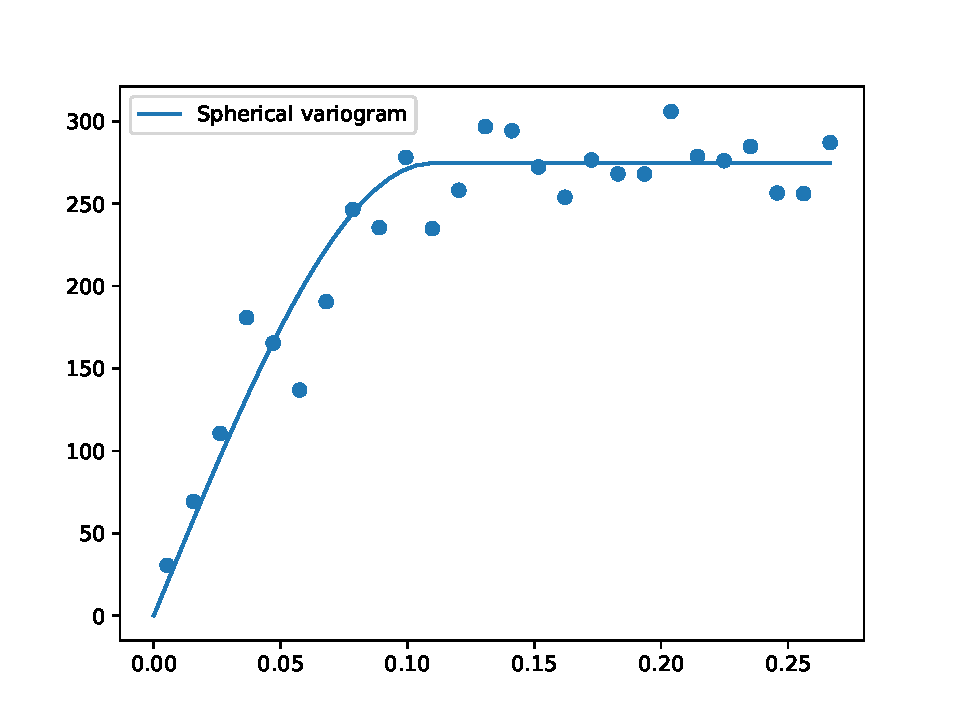
\includegraphics[width=0.4\textwidth]{graphics/variogram.pdf}
\caption{Fitted variogram}
\label{fig:variogram}
\end{figure}

\begin{figure*}[h!]
\centering
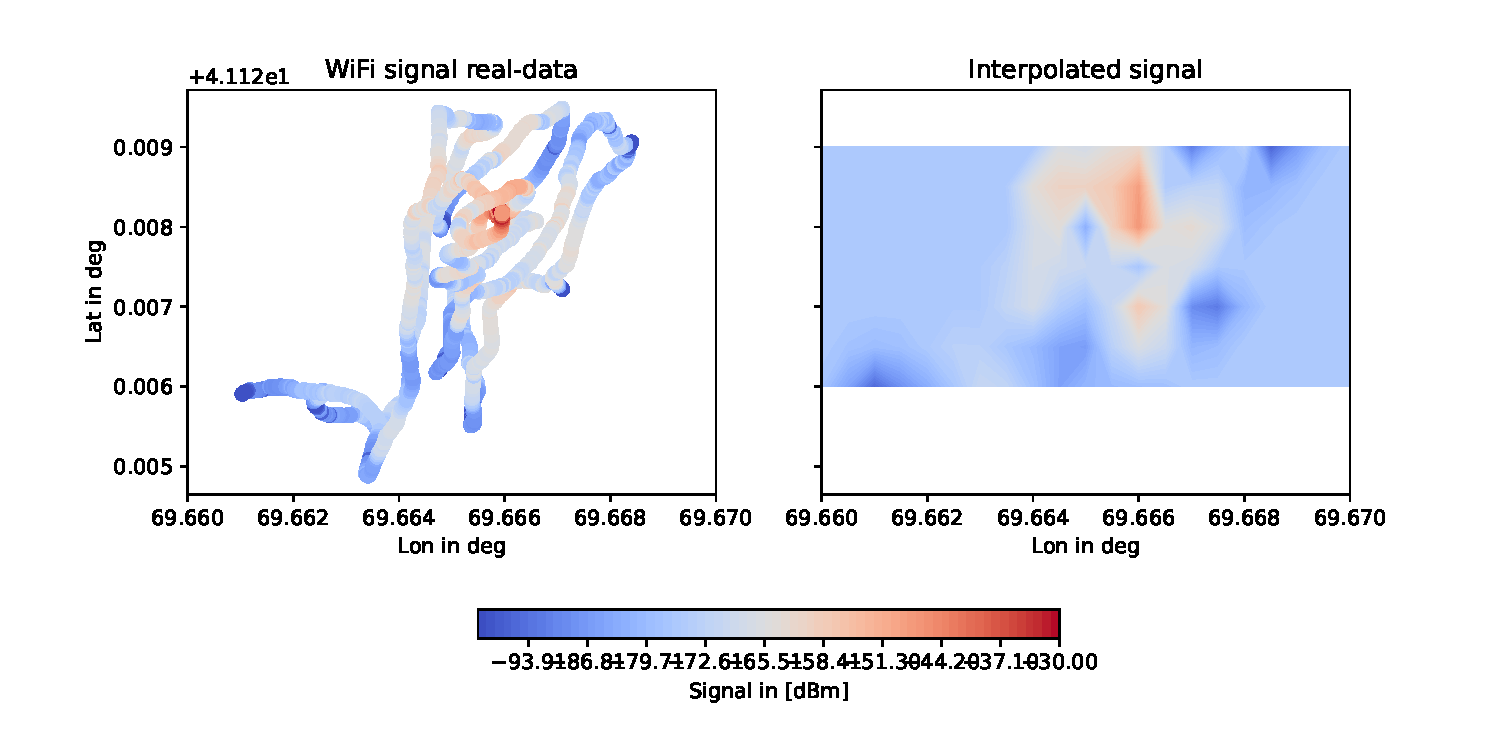
\includegraphics[width=0.8\textwidth]{graphics/estimate.pdf}
\caption{Actual and predicted data}
\label{fig:heatmap}
\end{figure*}


But since the values have $0$ means we can rewrite the above equation as follows:

$\min \sum_{i=1}^{n}\sum_{j=1}^{n}\lambda_i\lambda_j\sigma_{ij}-2\sum_{i=1}^{n}\lambda_i\sigma_{i0} + \sigma^2_{0}$

But we want to minimize the above expression so we need to find the derivative of the above formula and 
equate it to $0$. We then need to solve the following system of equations to find all $\lambda$'s:

$$
\begin{bmatrix}
\sigma_{11} & \ldots & \sigma_{1n} \\
\vdots  & \ddots & \vdots \\
\sigma_{n1} & \ldots & \sigma_{nn}
\end{bmatrix}
\begin{bmatrix}
\lambda_1\\
\vdots \\
\lambda_n
\end{bmatrix}
=
\begin{bmatrix}
\sigma_{10}\\
\vdots \\
\sigma_{n0}
\end{bmatrix}
$$


To compute the variogram and predict the values using Ordinary Kriging we have used the GSTools library~\cite{gstools}.
We have fitted spherical  variogram into the data. The result is shown in Figure~\ref{fig:variogram}.



We then estimated the values for signal strengths at unknown locations using the spherical variogram and Ordinary Kriging. 
The results are shown in Figure~\ref{fig:heatmap}.



